% Hình và bảng tra cứu chuyển từ thân báo cáo xuống; thân báo cáo trỏ tới bằng \ref.

\section*{Phụ lục P. Số liệu chương trình OCOP}
\label{apdx:ocop}
\addcontentsline{toc}{section}{Phụ lục P. Số liệu chương trình OCOP}

Hình~\ref{fig:ocop} bổ trợ cho mục~\ref{sec:boicanhchinhsach}.

\begin{figure}[H]
\centering
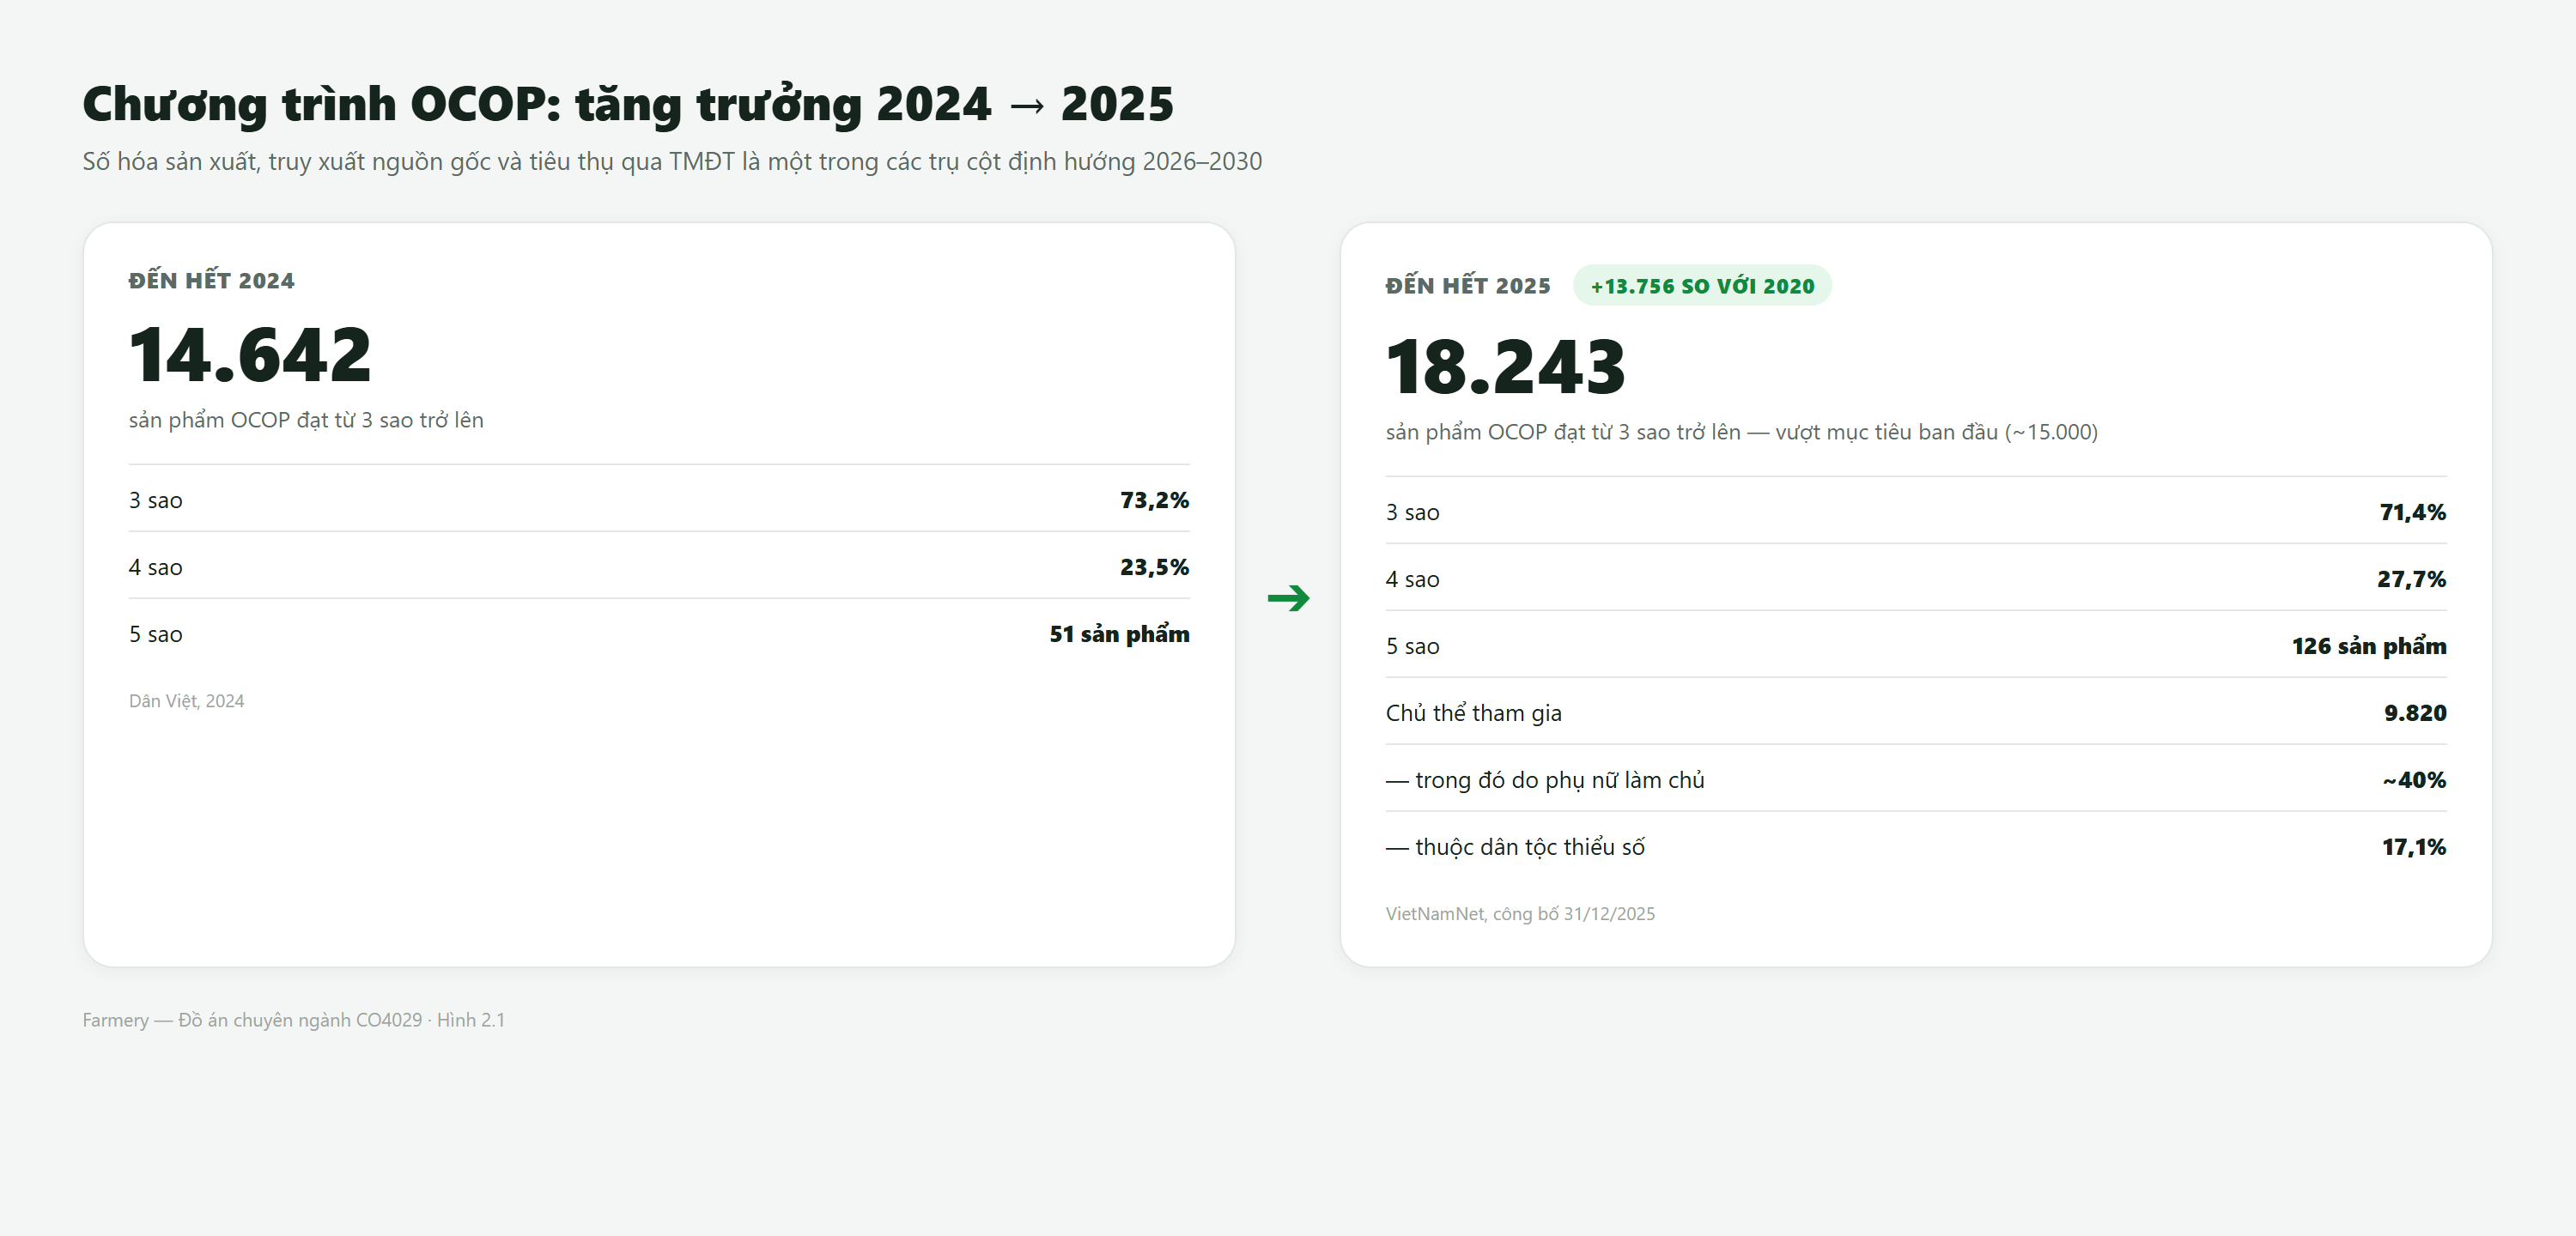
\includegraphics[width=\textwidth]{image/comparison/ocop-2024-2025.png}
\caption{Tăng trưởng của chương trình OCOP giai đoạn 2024--2025}
\label{fig:ocop}
\end{figure}

\clearpage
\section*{Phụ lục Q. Bản đồ hành trình khách hàng và nguồn giao dịch kho}
\label{apdx:hanhtrinh-kho}
\addcontentsline{toc}{section}{Phụ lục Q. Bản đồ hành trình khách hàng và nguồn giao dịch kho}

Hai bảng bổ trợ cho Chương~\ref{chap:hethong}: Bảng~\ref{tab:customer-journey} cho mục~\ref{subsec:customer-journey}, Bảng~\ref{tab:nguon-giaodich} cho phần lô, dòng tồn và sổ nhập xuất tại mục~\ref{sec:quytrinhnghiepvu}.

\begingroup
\tblsetup\tblzebra
\begin{longtable}{L{2.15cm} L{3.77cm} L{3.77cm} L{4.85cm}}
\caption{Bản đồ hành trình khách hàng trên hệ thống Farmery}
\label{tab:customer-journey} \\
\toprule
\rowcolor{tblheadbg}
\textbf{Giai đoạn} & \textbf{Luồng bán lẻ --- 1P} & \textbf{Luồng bán sỉ --- 3P} & \textbf{Điểm chạm} \\
\midrule
\endfirsthead
\toprule
\rowcolor{tblheadbg}
\textbf{Giai đoạn} & \textbf{Luồng bán lẻ --- 1P} & \textbf{Luồng bán sỉ --- 3P} & \textbf{Điểm chạm} \\
\midrule
\endhead
\bottomrule
\endfoot
\textbf{1. Khám phá} &
Tìm nông sản sạch theo danh mục, khu vực hoặc gợi ý cá nhân hóa trên trang chủ. &
Tìm nhà cung ứng có sản lượng lớn, tra cứu hồ sơ năng lực và chứng chỉ VietGAP/GlobalGAP. &
Web trên điện thoại, Trang chủ, Tìm kiếm theo ngữ nghĩa, Bộ lọc đa tiêu chí, Gợi ý sản phẩm tương tự.\\
\textbf{2. Cân nhắc} &
Xem chi tiết sản phẩm, quét mã QR xem nhật ký canh tác của lô hàng, đọc đánh giá của người mua trước. &
So sánh bảng giá bậc/MOQ, gửi yêu cầu báo giá (RFQ) riêng biệt. &
Trang chi tiết SP, Modal nhật ký GS1/QR, Trình đàm phán RFQ trực tuyến.\\
\textbf{3. Giao dịch} &
Chọn khung giờ giao phù hợp hàng tươi, thanh toán qua VietQR hoặc khi nhận hàng, áp dụng mã giảm giá. &
Thống nhất điều khoản RFQ, xác nhận giao kết hợp đồng, tiền thanh toán đợt 1 được nền tảng giữ trung gian. &
Trang thanh toán, Cổng thanh toán, Ví trung gian giữ tiền -- escrow.\\
\textbf{4. Giao nhận} &
Theo dõi tiến độ vận đơn 3PL theo thời gian thực; kiểm tra độ tươi ngon khi nhận hàng; nếu không đạt thì Farmery chịu trách nhiệm đổi trả trực tiếp. &
Theo dõi nhiều đợt giao trên hợp đồng; kiểm định số lượng/chất lượng tại kho và xác nhận biên bản. &
Webhook tracking 3PL, Quản lý đợt giao, Giải ngân tiền giữ trung gian sau khi xác nhận hoàn tất hoặc hết hạn khiếu nại.\\
\textbf{5. Đánh giá \& Gắn kết} &
Để lại điểm số, hình ảnh đánh giá sản phẩm; nhận gợi ý mua lại khi đến chu kỳ tiêu thụ. &
Đánh giá mức độ tuân thủ hợp đồng của nhà cung cấp; tái ký hợp đồng cho mùa vụ mới. &
Phân hệ đánh giá và uy tín, thông báo chu kỳ mua lại.\\
\end{longtable}
\endgroup

\begingroup
\tblsetup\tblzebra
\begin{longtable}{L{1.18cm} L{5.76cm} L{3.64cm} L{3.96cm}}
\caption{Các nguồn giao dịch làm thay đổi tồn kho}
\label{tab:nguon-giaodich} \\
\toprule
\rowcolor{tblheadbg}
\textbf{Chiều} & \textbf{Nguồn giao dịch} & \textbf{Hàng của ai} & \textbf{Người thực hiện} \\
\midrule
\endfirsthead
\toprule
\rowcolor{tblheadbg}
\textbf{Chiều} & \textbf{Nguồn giao dịch} & \textbf{Hàng của ai} & \textbf{Người thực hiện} \\
\midrule
\endhead
\bottomrule
\endfoot
Nhập & Thu mua trực tiếp từ chào hàng của nhà cung cấp & Farmery & Nhân viên kho \\
Nhập & Thu mua lại lô bán sỉ cận hạn với giá chiết khấu & Farmery & Nhân viên thu mua, nhân viên kho \\
Nhập & Nhà cung cấp gửi hàng bán sỉ vào kho theo dịch vụ thuê kho & Nhà cung cấp & Nhân viên kho \\
Nhập & Hàng bán lẻ hoàn về do khách từ chối nhận hoặc giao thất bại & Farmery & Nhân viên kho \\
Nhập & Hàng đổi trả sau khiếu nại chất lượng & Farmery & Nhân viên kho \\
Xuất & Đơn bán lẻ & Farmery & Hệ thống giữ chỗ, nhân viên kho xuất \\
Xuất & Đợt giao của hợp đồng bán sỉ, lấy từ hàng gửi kho & Nhà cung cấp & Nhân viên kho \\
Xuất & Chào sỉ hàng tồn dư hoặc cận hạn của Farmery & Farmery & Nhân viên thu mua, nhân viên kho \\
Xuất & Hủy hàng do hỏng, hết hạn hoặc hao hụt & Cả hai & Nhân viên kho \\
Xuất & Trả lại nhà cung cấp: bị từ chối khi kiểm định, hoặc rút hàng gửi kho & Nhà cung cấp & Nhân viên kho \\
Giữ & Giữ chỗ khi đơn chờ thanh toán, nhả khi đơn bị hủy hoặc quá hạn & Farmery & Hệ thống \\
Đổi & Sơ chế, phân loại, đóng gói --- đổi số lượng và đơn vị bán ngay trong kho & Cả hai & Nhân viên kho \\
Đổi & Đổi chủ tại chỗ --- hàng gửi kho được Farmery thu mua lại & Nhà cung cấp sang Farmery & Nhân viên thu mua \\
Khóa & Thu hồi lô --- khóa mọi dòng tồn của lô ở cả hai luồng & Cả hai & Kiểm duyệt viên \\
Chỉnh & Kiểm kê, điều chỉnh khi lệch số thực tế & Cả hai & Nhân viên kho \\
\end{longtable}
\endgroup

\clearpage
\section*{Phụ lục R. Lưu đồ quy trình nghiệp vụ chi tiết}
\label{apdx:luudo}
\addcontentsline{toc}{section}{Phụ lục R. Lưu đồ quy trình nghiệp vụ chi tiết}

Bảy lưu đồ dưới đây bổ trợ mục~\ref{subsec:mohinhquytrinh}, dùng ký hiệu tại Hình~\ref{fig:chu-thich-flowchart}.

\clearpage
\begin{figure}[p]
\centering
\begin{adjustbox}{max totalsize={\textwidth}{\dimexpr\textheight-2.4cm\relax},center}
\begin{tikzpicture}[farm/chart]
    \node[farm/terminal] (start) at (0,0) {Bắt đầu};
    \node[farm/process] (register) at (0,-1.25) {Nhà bán: đăng ký, khai báo định danh và thông tin trang trại};
    \node[farm/process] (otp) at (0,-2.75) {Hệ thống gửi OTP;\\nhà bán nhập mã xác thực};
    \node[farm/decision] (valid) at (0,-4.5) {OTP hợp lệ?};
    \node[farm/decision] (attempts) at (6,-4.5) {Sai quá 5 lần?};
    \node[farm/exception] (lock) at (6,-6.4) {Hệ thống: khóa tạm thời\\30 phút};
    \node[farm/process] (ekyc) at (0,-6.75) {Nhà bán: xác minh danh tính điện tử (eKYC) --- ảnh giấy tờ định danh và ảnh chân dung};
    \node[farm/process] (evidence) at (0,-8.55) {Nhà bán: tải chứng nhận (nếu có), mã số, cơ quan cấp và hạn dùng};
    \node[farm/process] (review) at (0,-10.4) {Kiểm duyệt: đối chiếu kết quả eKYC và chứng nhận với cơ quan cấp hoặc kiểm tra thủ công};
    \node[farm/decision] (approved) at (0,-12.45) {eKYC và hồ sơ\\đạt yêu cầu?};
    \node[farm/processnarrow] (supplement) at (6,-12.45) {Hệ thống: thông báo lý do của bước không đạt; nhà bán bổ sung};
    \node[farm/process] (verified) at (0,-14.75) {Hệ thống: trạng thái ``Đã xác thực'', kích hoạt quyền đăng bán; gắn nhãn chứng nhận nếu có};
    \node[farm/process] (monitor) at (0,-16.45) {Hệ thống: theo dõi hiệu lực chứng nhận trong quá trình hoạt động};
    \node[farm/processnarrow] (expiry) at (6,-16.45) {Còn dưới 30 ngày: nhắc gia hạn.\\Hết hạn: ẩn nhãn đến khi cập nhật; không gỡ sản phẩm.};
    \node[farm/terminal] (finish) at (0,-18.1) {Hoàn tất đăng ký};
    \node[farm/note] at (2.7,-19.9) {\textbf{Ngoại lệ xuyên suốt:} nếu phát hiện chứng nhận giả mạo qua xác minh hoặc khiếu nại, khóa vĩnh viễn tài khoản, ghi vào danh sách vi phạm và chặn đăng ký lại bằng cùng thông tin định danh.};
    \foreach \source/\target in {start/register,register/otp,otp/valid,ekyc/evidence,evidence/review,review/approved,verified/monitor,monitor/finish}
        \draw[farm/arrow] (\source) -- (\target);
    \draw[farm/arrow] (valid) -- node[farm/label,right] {Có} (ekyc);
    \draw[farm/arrow] (valid) -- node[farm/label,above] {Không} (attempts);
    \draw[farm/arrow] (attempts.north) |- node[farm/label,near start,right] {Không: nhập lại} (otp.east);
    \draw[farm/arrow] (attempts) -- node[farm/label,right] {Có} (lock);
    \draw[farm/arrow] (lock.east) -- (8.6,-6.4) -- (8.6,-1.8) -| node[farm/label,near start,above] {Sau 30 phút} (otp.north);
    \draw[farm/arrow] (approved) -- node[farm/label,right] {Có} (verified);
    \draw[farm/arrow] (approved) -- node[farm/label,above] {Không} (supplement);
    \draw[farm/arrow] (supplement.west) -- (3.3,-12.45) -- (3.3,-6.75) -- (ekyc.east);
    \draw[farm/arrow,dashed] (monitor) -- (expiry);
\end{tikzpicture}
\end{adjustbox}
\caption{Flowchart đăng ký và xác thực nhà bán, kiểm duyệt chứng nhận.}
\label{fig:flow-dang-ky}
\end{figure}
\clearpage
\clearpage
\clearpage
\begin{figure}[p]
\centering
\begin{adjustbox}{max totalsize={\textwidth}{\dimexpr\textheight-2.4cm\relax},center}
\begin{tikzpicture}[farm/chart]
    \node[farm/terminal] (start) at (0,0) {Nhà bán đã xác thực};
    \node[farm/process] (create) at (0,-1.5) {Nhà bán: tạo sản phẩm, khai báo giá lẻ/sỉ, sản lượng, ngày thu hoạch và nhật ký theo lô};
    \node[farm/decision] (complete) at (0,-3.6) {Có nhật ký gần nhất\\và ảnh thực tế?};
    \node[farm/processnarrow] (supplement) at (6,-3.6) {Nhà bán: bổ sung nhật ký và hình ảnh còn thiếu};
    \node[farm/process] (automatic) at (0,-5.6) {Hệ thống: kiểm tra ảnh trùng lặp, từ khóa cấm và giá bất thường};
    \node[farm/decision] (passed) at (0,-7.4) {Đạt kiểm tra\\sơ bộ?};
    \node[farm/processnarrow] (revise) at (6,-7.4) {Chưa duyệt; nhà bán chỉnh sửa thông tin sản phẩm};
    \node[farm/decision] (trusted) at (0,-9.9) {Uy tín nhà bán\\$\geq 80/100$?};
    \node[farm/processnarrow] (manual) at (6,-9.9) {Kiểm duyệt: kiểm tra thủ công sản phẩm mới / nhà bán chưa có lịch sử giao dịch};
    \node[farm/decision] (accepted) at (6,-12.4) {Được duyệt?};
    \node[farm/process] (publish) at (0,-12.4) {Hệ thống: duyệt, công khai sản phẩm; sinh QR riêng cho lô, liên kết hồ sơ, chứng nhận, nhật ký và vận chuyển};
    \node[farm/decision] (changed) at (0,-14.6) {Thay đổi\\trọng yếu?};
    \node[farm/processnarrow] (pending) at (6,-14.6) {Giá thay đổi vượt 20\% hoặc đổi mô tả chất lượng:\\chuyển chờ duyệt lại};
    \node[farm/terminal] (finish) at (0,-16.6) {Tiếp tục hiển thị};
    \node[farm/connector] (reviseout) at (9,-7.4) {A};
    \node[farm/connector] (revisein) at (6,-0.2) {A};
    \node[farm/connector] (reviewout) at (9,-14.6) {B};
    \node[farm/connector] (reviewin) at (6,-5.6) {B};
    \node[farm/note] at (2.7,-18.6) {\textbf{Cập nhật nhỏ:} thay đổi còn hàng/hết hàng không cần duyệt lại. Nhánh hậu kiểm nhanh chỉ áp dụng cho nhà bán đạt điểm uy tín từ 80/100 trở lên (mục~\ref{subsec:danhgianghiepvu}); việc kiểm tra được thực hiện sau khi công khai sản phẩm.\\[2pt]\textbf{Điểm nối:} vòng tròn A quay lại bước tạo/chỉnh sửa sản phẩm, vòng tròn B quay lại bước kiểm tra tự động --- quy ước ký hiệu xem Hình~\ref{fig:chu-thich-flowchart}.};
    \foreach \source/\target in {start/create,create/complete,automatic/passed,manual/accepted,publish/changed}
        \draw[farm/arrow] (\source) -- (\target);
    \draw[farm/arrow] (complete) -- node[farm/label,right] {Có} (automatic);
    \draw[farm/arrow] (complete) -- node[farm/label,above] {Không} (supplement);
    \draw[farm/arrow] (supplement.north) |- (create.east);
    \draw[farm/arrow] (passed) -- node[farm/label,right] {Có} (trusted);
    \draw[farm/arrow] (passed) -- node[farm/label,above] {Không} (revise);
    \draw[farm/arrow] (revise) -- (reviseout);
    \draw[farm/arrow] (revisein.south) |- (create.east);
    \draw[farm/arrow] (trusted) -- node[farm/label,right] {Có} (publish);
    \draw[farm/arrow] (trusted) -- node[farm/label,above] {Không} (manual);
    \draw[farm/arrow] (accepted) -- node[farm/label,above] {Có} (publish);
    \draw[farm/arrow] (accepted.east) -- node[farm/label,below,near start] {Không} (8.6,-12.4) -- (8.6,-8.6) -- (6,-8.6) -- (revise.south);
    \draw[farm/arrow] (changed) -- node[farm/label,right] {Không} (finish);
    \draw[farm/arrow] (changed) -- node[farm/label,above] {Có} (pending);
    \draw[farm/arrow] (pending) -- (reviewout);
    \draw[farm/arrow] (reviewin) -- (automatic);
\end{tikzpicture}
\end{adjustbox}
\caption{Flowchart đăng và kiểm duyệt sản phẩm, sinh mã QR truy xuất.}
\label{fig:flow-san-pham}
\end{figure}
\clearpage
\clearpage
\begin{figure}[H]
\centering
\begin{adjustbox}{max totalsize={\textwidth}{\dimexpr\textheight-4.6cm\relax},center}
\begin{tikzpicture}[farm/chart]
    \node[farm/connector] (connA) at (0,0) {A};
    \node[farm/processnarrow] (connAnote) at (3.4,0) {Tiếp nối vòng tròn \textbf{A} của Hình~\ref{fig:flow-ban-le-a} (đơn đã xác nhận)};
    \node[farm/process] (ship) at (0,-2) {Nhân viên kho: đóng gói hàng dễ hư hỏng, bàn giao đơn vị vận chuyển hoặc nhân viên giao hàng};
    \node[farm/decision] (refused) at (0,-4.1) {Người nhận\\từ chối COD?};
    \node[farm/exception] (return) at (6.5,-4.1) {Hoàn hàng về kho; đánh giá lại chất lượng lô trước khi quyết định bán tiếp hay hủy};
    \node[farm/process] (receive) at (0,-6.4) {Khách lẻ: xác nhận nhận hàng và đánh giá sản phẩm trong thời hạn quy định};
    \node[farm/process] (sellerdone) at (0,-8.4) {Hệ thống: đơn hoàn tất, ghi nhận doanh thu và biên lợi nhuận của lô};
    \node[farm/terminal] (finish) at (0,-10.3) {Kết thúc};
    \node[farm/note] at (2.7,-12) {\textbf{Hàng không đạt:} Farmery chịu trách nhiệm đổi trả trực tiếp với khách lẻ, sau đó mới đối chiếu lại với nhà cung cấp gốc nếu lỗi thuộc khâu cung ứng (Hình~\ref{fig:flow-van-chuyen}).};
    \foreach \source/\target in {connA/ship,ship/refused,receive/sellerdone,sellerdone/finish}
        \draw[farm/arrow] (\source) -- (\target);
    \draw[farm/arrow,dashed] (connAnote) -- (connA);
    \draw[farm/arrow] (refused) -- node[farm/label,right] {Không} (receive);
    \draw[farm/arrow] (refused) -- node[farm/label,above] {Có} (return);
    \draw[farm/arrow] (return.south) |- (finish.east);
\end{tikzpicture}
\end{adjustbox}
\caption[Lưu đồ quy trình bán lẻ B2C (phần 2)]{Lưu đồ quy trình bán lẻ B2C (phần 2): giao hàng, nhận hàng và hoàn tất đơn}
\label{fig:flow-ban-le-b}
\end{figure}

\clearpage
\begin{figure}[H]
\centering
\begin{adjustbox}{max totalsize={\textwidth}{\dimexpr\textheight-4.6cm\relax},center}
\begin{tikzpicture}[farm/chart]
    \node[farm/terminal] (start) at (0,0) {Đơn hàng bán lẻ hoàn tất (verified purchase)};
    \node[farm/decision] (window) at (0,-2) {Trong thời hạn\\đánh giá quy định?};
    \node[farm/exception] (locked) at (6,-2) {Hệ thống: khóa chức năng đánh giá cho đơn này};
    \node[farm/process] (submit) at (0,-4.2) {Người mua: gửi đánh giá (sao 1--5, bình luận, ảnh minh chứng)};
    \node[farm/process] (autocheck) at (0,-6) {Hệ thống: kiểm duyệt tự động sơ bộ + mô-đun AI phát hiện bất thường};
    \node[farm/decision] (suspect) at (0,-8.2) {Nghi ngờ\\giả/spam?};
    \node[farm/process] (manual) at (6,-8.2) {Kiểm duyệt viên: xem xét thủ công};
    \node[farm/decision] (approved) at (6,-10.6) {Được duyệt?};
    \node[farm/exception] (reject) at (6,-13) {Ẩn đánh giá, thông báo lý do cho người mua};
    \node[farm/process] (publish) at (0,-10.6) {Hệ thống: công khai đánh giá};
    \node[farm/process] (score) at (0,-12.6) {Hệ thống: cập nhật điểm uy tín tổng hợp của nhà cung cấp (thang 0--100)};
    \node[farm/process] (reply) at (0,-14.6) {Nhà cung cấp: có thể phản hồi công khai (một lần) dưới đánh giá};
    \node[farm/decision] (threshold) at (0,-16.8) {Điểm uy tín\\$\geq 80/100$?};
    \node[farm/processnarrow] (perks) at (6,-16.8) {Nhà cung cấp: đủ điều kiện hậu kiểm nhanh và ưu tiên hiển thị theo uy tín (miễn phí)};
    \node[farm/terminal] (finish) at (0,-19.2) {Kết thúc};
    \node[farm/note] at (2.7,-21.2) {\textbf{Điểm uy tín:} chuẩn hóa về thang 0--100, tính bằng trung bình có trọng số điểm sao của các đánh giá hợp lệ trong 6 tháng gần nhất (đánh giá gần đây và đơn giá trị lớn có trọng số cao hơn), không tính đánh giá bị ẩn.\\[2pt]\textbf{Liên hệ:} mô-đun AI phát hiện bất thường tại mục~\ref{sec:thietkeAI}; điều kiện hậu kiểm nhanh tại mục~\ref{sec:quytrinhnghiepvu} (Đăng và kiểm duyệt sản phẩm).};
    \foreach \source/\target in {start/window,submit/autocheck,autocheck/suspect,publish/score,score/reply,reply/threshold,manual/approved}
        \draw[farm/arrow] (\source) -- (\target);
    \draw[farm/arrow] (window) -- node[farm/label,right] {Có} (submit);
    \draw[farm/arrow] (window) -- node[farm/label,above] {Không} (locked);
    \draw[farm/arrow] (suspect) -- node[farm/label,right] {Không} (publish);
    \draw[farm/arrow] (suspect) -- node[farm/label,above] {Có} (manual);
    \draw[farm/arrow] (approved) -- node[farm/label,right] {Không} (reject);
    \draw[farm/arrow] (approved.west) -- node[farm/label,above] {Có} (publish.east);
    \draw[farm/arrow] (threshold) -- node[farm/label,above] {Có} (perks);
    \draw[farm/arrow] (threshold) -- node[farm/label,right] {Không} (finish);
    % Ba nhánh kết thúc (hết hạn đánh giá, đánh giá bị ẩn, nhà cung cấp đạt ngưỡng)
    % gom vào một đường trục bên phải rồi mới vào nút Kết thúc, tránh cắt qua node.
    \draw[line width=0.7pt, draw=black!75] (locked.east) -- (9,-2);
    \draw[line width=0.7pt, draw=black!75] (reject.east) -- (9,-13);
    \draw[line width=0.7pt, draw=black!75] (perks.east) -- (9,-16.8);
    \draw[farm/arrow] (9,-2) -- (9,-19.2) -- (finish.east);
\end{tikzpicture}
\end{adjustbox}
\caption[Lưu đồ quy trình đánh giá sản phẩm và nhà cung cấp]{Lưu đồ quy trình đánh giá sản phẩm và nhà cung cấp: kiểm duyệt, cập nhật điểm uy tín và quyền lợi nhà cung cấp}
\label{fig:flow-danh-gia}
\end{figure}

\clearpage
\clearpage
\begin{figure}[p]
\centering
\begin{adjustbox}{max totalsize={\textwidth}{\dimexpr\textheight-2.4cm\relax},center}
\begin{tikzpicture}[farm/chart]
    \node[farm/connector] (connA) at (0,0) {A};
    \node[farm/processnarrow] (connAnote) at (3.9,0) {Tiếp nối vòng tròn \textbf{A} của Hình~\ref{fig:flow-ban-si-a} (hợp đồng vừa được ký)};
    \draw[farm/arrow,dashed] (connAnote) -- (connA);
    \node[farm/decision] (escrowq) at (0,-2) {Giá trị vượt ngưỡng\\ký quỹ (FR7.4)?};
    \node[farm/processnarrow] (nonescrow) at (6,-2) {Không ký quỹ: thanh toán theo kỳ hạn công nợ đã thỏa thuận};
    \node[farm/process] (escrow) at (0,-4.3) {Bên mua nộp tiền đợt giao vào tài khoản ký quỹ tại cổng thanh toán trung gian; hệ thống ghi nhận trạng thái ``đã ký quỹ''};
    \node[farm/process] (delivery) at (0,-6.7) {Nhà bán giao theo từng đợt; hệ thống lập hóa đơn và cập nhật sổ công nợ};
    \node[farm/process] (settle) at (0,-8.7) {Doanh nghiệp: xác nhận số lượng và chất lượng của đợt giao};
    \node[farm/process] (release) at (0,-10.7) {Hệ thống: ghi nhận thanh toán; nếu có ký quỹ thì ra lệnh cổng trung gian giải ngân khoản đã giữ cho nhà bán};
    \node[farm/decision] (complete) at (0,-13.1) {Còn đợt giao\\theo hợp đồng?};
    \node[farm/processnarrow] (reconcile) at (6,-13.1) {Hai bên: đối soát, hoàn tất thanh toán công nợ theo kỳ hạn};
    \node[farm/process] (sellerdone) at (0,-15.3) {Nhà bán: hợp đồng hoàn tất --- hệ thống cập nhật doanh thu và lịch sử bán sỉ};
    \node[farm/terminal] (finish) at (0,-17.1) {Hoàn tất hợp đồng};
    \node[farm/exception,text width=3.8cm] (exceptions) at (6,-7.6) {\textbf{Ngoại lệ hợp đồng}\\[3pt]Giao thiếu / trễ: áp dụng phạt và ghi lịch sử uy tín.\\[4pt]Quá hạn công nợ: nhắc tự động; có thể khóa RFQ mới đến khi trả đủ.\\[4pt]Hủy giữa kỳ: xử lý theo điều khoản hủy đã ký.\\[4pt]Tranh chấp đợt đã ký quỹ: giữ nguyên khoản ký quỹ tại cổng trung gian đến khi xử lý xong khiếu nại.};
    \foreach \source/\target in {connA/escrowq,escrow/delivery,delivery/settle,settle/release,release/complete,sellerdone/finish}
        \draw[farm/arrow] (\source) -- (\target);
    \draw[farm/arrow] (escrowq) -- node[farm/label,right] {Có} (escrow);
    \draw[farm/arrow] (escrowq) -- node[farm/label,above] {Không} (nonescrow);
    % Đi vòng qua rãnh trống x=3.3 để không cắt ngang hộp ngoại lệ đặt tại x=6.
    \draw[farm/arrow] (nonescrow.west) -- (3.3,-2) -- (3.3,-6.7) -- (delivery.east);
    \draw[farm/arrow] (complete) -- node[farm/label,above] {Không} (reconcile);
    \draw[farm/arrow] (reconcile.south) |- (sellerdone.east);
    \draw[farm/arrow] (complete.west) -- (-3.5,-13.1) |- node[farm/label,near start,left] {Có} (delivery.west);
    \draw[farm/arrow,dashed] (delivery) -- (exceptions);
\end{tikzpicture}
\end{adjustbox}
\caption{Flowchart bán sỉ (B2B) --- phần 2: ký quỹ trung gian, giao hàng theo đợt, giải ngân và công nợ.}
\label{fig:flow-ban-si-b}
\end{figure}
\clearpage

\clearpage
\begin{figure}[H]
\centering
\begin{adjustbox}{max totalsize={\textwidth}{\dimexpr\textheight-4.6cm\relax},center}
\begin{tikzpicture}[farm/chart]
    \node[farm/terminal] (start) at (0,0) {Đơn hàng dự kiến};
    \node[farm/process] (method) at (0,-1.35) {Hệ thống: ưu tiên giao nhanh / bảo quản lạnh theo danh mục dễ hư hỏng};
    \node[farm/decision] (unsafe) at (0,-3.2) {Thời gian giao vượt ngưỡng an toàn?};
    \node[farm/processnarrow] (warn) at (6,-3.2) {Hệ thống: cảnh báo trước khi khách xác nhận đặt hàng};
    \node[farm/process] (confirm) at (0,-5.6) {Khách xác nhận đặt hàng;\\bên giữ hàng (nhà cung cấp hoặc nhân viên kho) đóng gói theo nhiệt độ, độ ẩm và vật liệu phù hợp};
    \node[farm/process] (transport) at (0,-7.3) {Đơn vị vận chuyển hoặc nhân viên giao hàng của Farmery: giao hàng, cập nhật trạng thái theo thời gian thực};
    \node[farm/decision] (damage) at (0,-9.4) {Người nhận kiểm tra: hàng hư hỏng?};
    \node[farm/terminal] (received) at (6,-9.4) {Nhận hàng, hoàn tất};
    \node[farm/process] (claim) at (0,-11.4) {Người nhận: khiếu nại trong thời hạn, kèm ảnh / video minh chứng};
    \node[farm/decision] (suspicious) at (0,-13.4) {Người mua có\\dấu hiệu bất thường?};
    \node[farm/processnarrow] (manual) at (6,-13.4) {Nhân viên vận hành: xem xét thủ công trước khi quyết định hoàn tiền};
    \node[farm/process] (classify) at (0,-15.8) {Hệ thống: phân loại nguyên nhân từ nhà cung cấp, vận chuyển hoặc bảo quản của người nhận};
    \node[farm/process] (resolve) at (0,-17.7) {Nhân viên vận hành: hoàn tiền toàn phần / một phần, đổi lô mới hoặc từ chối nếu thiếu bằng chứng};
    \node[farm/terminal] (finish) at (0,-19.4) {Thông báo kết quả xử lý};
    \node[farm/exception] (repeated) at (6,-17.6) {Khiếu nại lặp lại từ cùng nhà cung cấp trong thời gian ngắn:\\gắn cờ và tạm hạ ưu tiên hiển thị đến khi rà soát};
    \foreach \source/\target in {start/method,method/unsafe,confirm/transport,transport/damage,claim/suspicious,classify/resolve,resolve/finish}
        \draw[farm/arrow] (\source) -- (\target);
    \draw[farm/arrow] (unsafe) -- node[farm/label,right] {Không} (confirm);
    \draw[farm/arrow] (unsafe) -- node[farm/label,above] {Có} (warn);
    \draw[farm/arrow] (warn.south) |- (confirm.east);
    \draw[farm/arrow] (damage) -- node[farm/label,right] {Có} (claim);
    \draw[farm/arrow] (damage) -- node[farm/label,above] {Không} (received);
    \draw[farm/arrow] (suspicious) -- node[farm/label,right] {Không} (classify);
    \draw[farm/arrow] (suspicious) -- node[farm/label,above] {Có} (manual);
    \draw[farm/arrow] (manual.south) |- (classify.east);
    \draw[farm/arrow,dashed] (resolve) -- (repeated);
\end{tikzpicture}
\end{adjustbox}
\caption{Lưu đồ quy trình vận chuyển hàng dễ hư hỏng và xử lý khiếu nại}
\label{fig:flow-van-chuyen}
\end{figure}
\clearpage
\begin{figure}[H]
\centering
\begin{adjustbox}{max totalsize={\textwidth}{\dimexpr\textheight-4.6cm\relax},center}
\begin{tikzpicture}[farm/chart]
    \node[farm/terminal] (start) at (0,0) {Bắt đầu đợt giám sát};
    \node[farm/process] (review) at (0,-1.5) {Kiểm duyệt viên: kiểm duyệt hồ sơ mới, sản phẩm mới / thay đổi trọng yếu và chứng nhận sắp hết hạn};
    \node[farm/process] (monitor) at (0,-3.2) {Nhân viên vận hành: theo dõi cảnh báo tỷ lệ khiếu nại bất thường và giao dịch có nguy cơ gian lận};
    \node[farm/decision] (violation) at (0,-5.2) {Phát hiện\\vi phạm?};
    \node[farm/decision] (severe) at (0,-7.9) {Vi phạm\\nghiêm trọng?};
    \node[farm/exception] (lock) at (6,-7.9) {Giả mạo chứng nhận / gian lận:\\khóa ngay tài khoản, không qua nhắc nhở trung gian};
    \node[farm/process] (sanction) at (0,-10.5) {Kiểm duyệt viên / nhân viên vận hành: xử lý theo mức độ và số lần vi phạm: nhắc nhở, cảnh cáo công khai, tạm khóa hoặc khóa vĩnh viễn};
    \node[farm/exception] (orders) at (6,-10.5) {Rà soát toàn bộ đơn đang xử lý của tài khoản, bảo vệ khách đã đặt trước};
    \node[farm/process] (audit) at (0,-12.7) {Hệ thống: ghi nhật ký thao tác kèm người xử lý, lý do và quyết định};
    \node[farm/process] (report) at (0,-14.5) {Nhân viên vận hành: truy xuất báo cáo định kỳ, hỗ trợ quyết định vận hành và báo cáo các bên liên quan};
    \node[farm/terminal] (finish) at (0,-16.2) {Kết thúc đợt giám sát};
    \node[farm/note] at (2.7,-18) {\textbf{Nguyên tắc phân cấp:} các hình thức xử lý được lựa chọn theo mức độ và số lần vi phạm, không bắt buộc đi qua mọi mức. Quy trình giám sát được thực hiện định kỳ; trường hợp nghiêm trọng được xử lý ngay khi phát hiện.};
    \foreach \source/\target in {start/review,review/monitor,monitor/violation,lock/orders,sanction/audit,audit/report,report/finish}
        \draw[farm/arrow] (\source) -- (\target);
    \draw[farm/arrow] (violation) -- node[farm/label,right] {Có} (severe);
    \draw[farm/arrow] (violation.west) -- (-3.6,-5.2) |- node[farm/label,near start,left] {Không} (report.west);
    \draw[farm/arrow] (severe) -- node[farm/label,right] {Không} (sanction);
    \draw[farm/arrow] (severe) -- node[farm/label,above] {Có} (lock);
    \draw[farm/arrow] (orders.south) |- (audit.east);
\end{tikzpicture}
\end{adjustbox}
\caption{Lưu đồ quy trình giám sát, xử lý vi phạm và báo cáo của nhân sự nội bộ}
\label{fig:flow-quan-tri}
\end{figure}

\clearpage
\section*{Phụ lục S. Sơ đồ và đặc tả use case chi tiết}
\label{apdx:usecase}
\addcontentsline{toc}{section}{Phụ lục S. Sơ đồ và đặc tả use case chi tiết}

Các sơ đồ và bảng đặc tả dưới đây bổ trợ mục~\ref{sec:sddchitiet}.

\begin{figure}[p]
\centering
\begin{adjustbox}{max totalsize={\textwidth}{\dimexpr\textheight-2.5cm\relax},center}
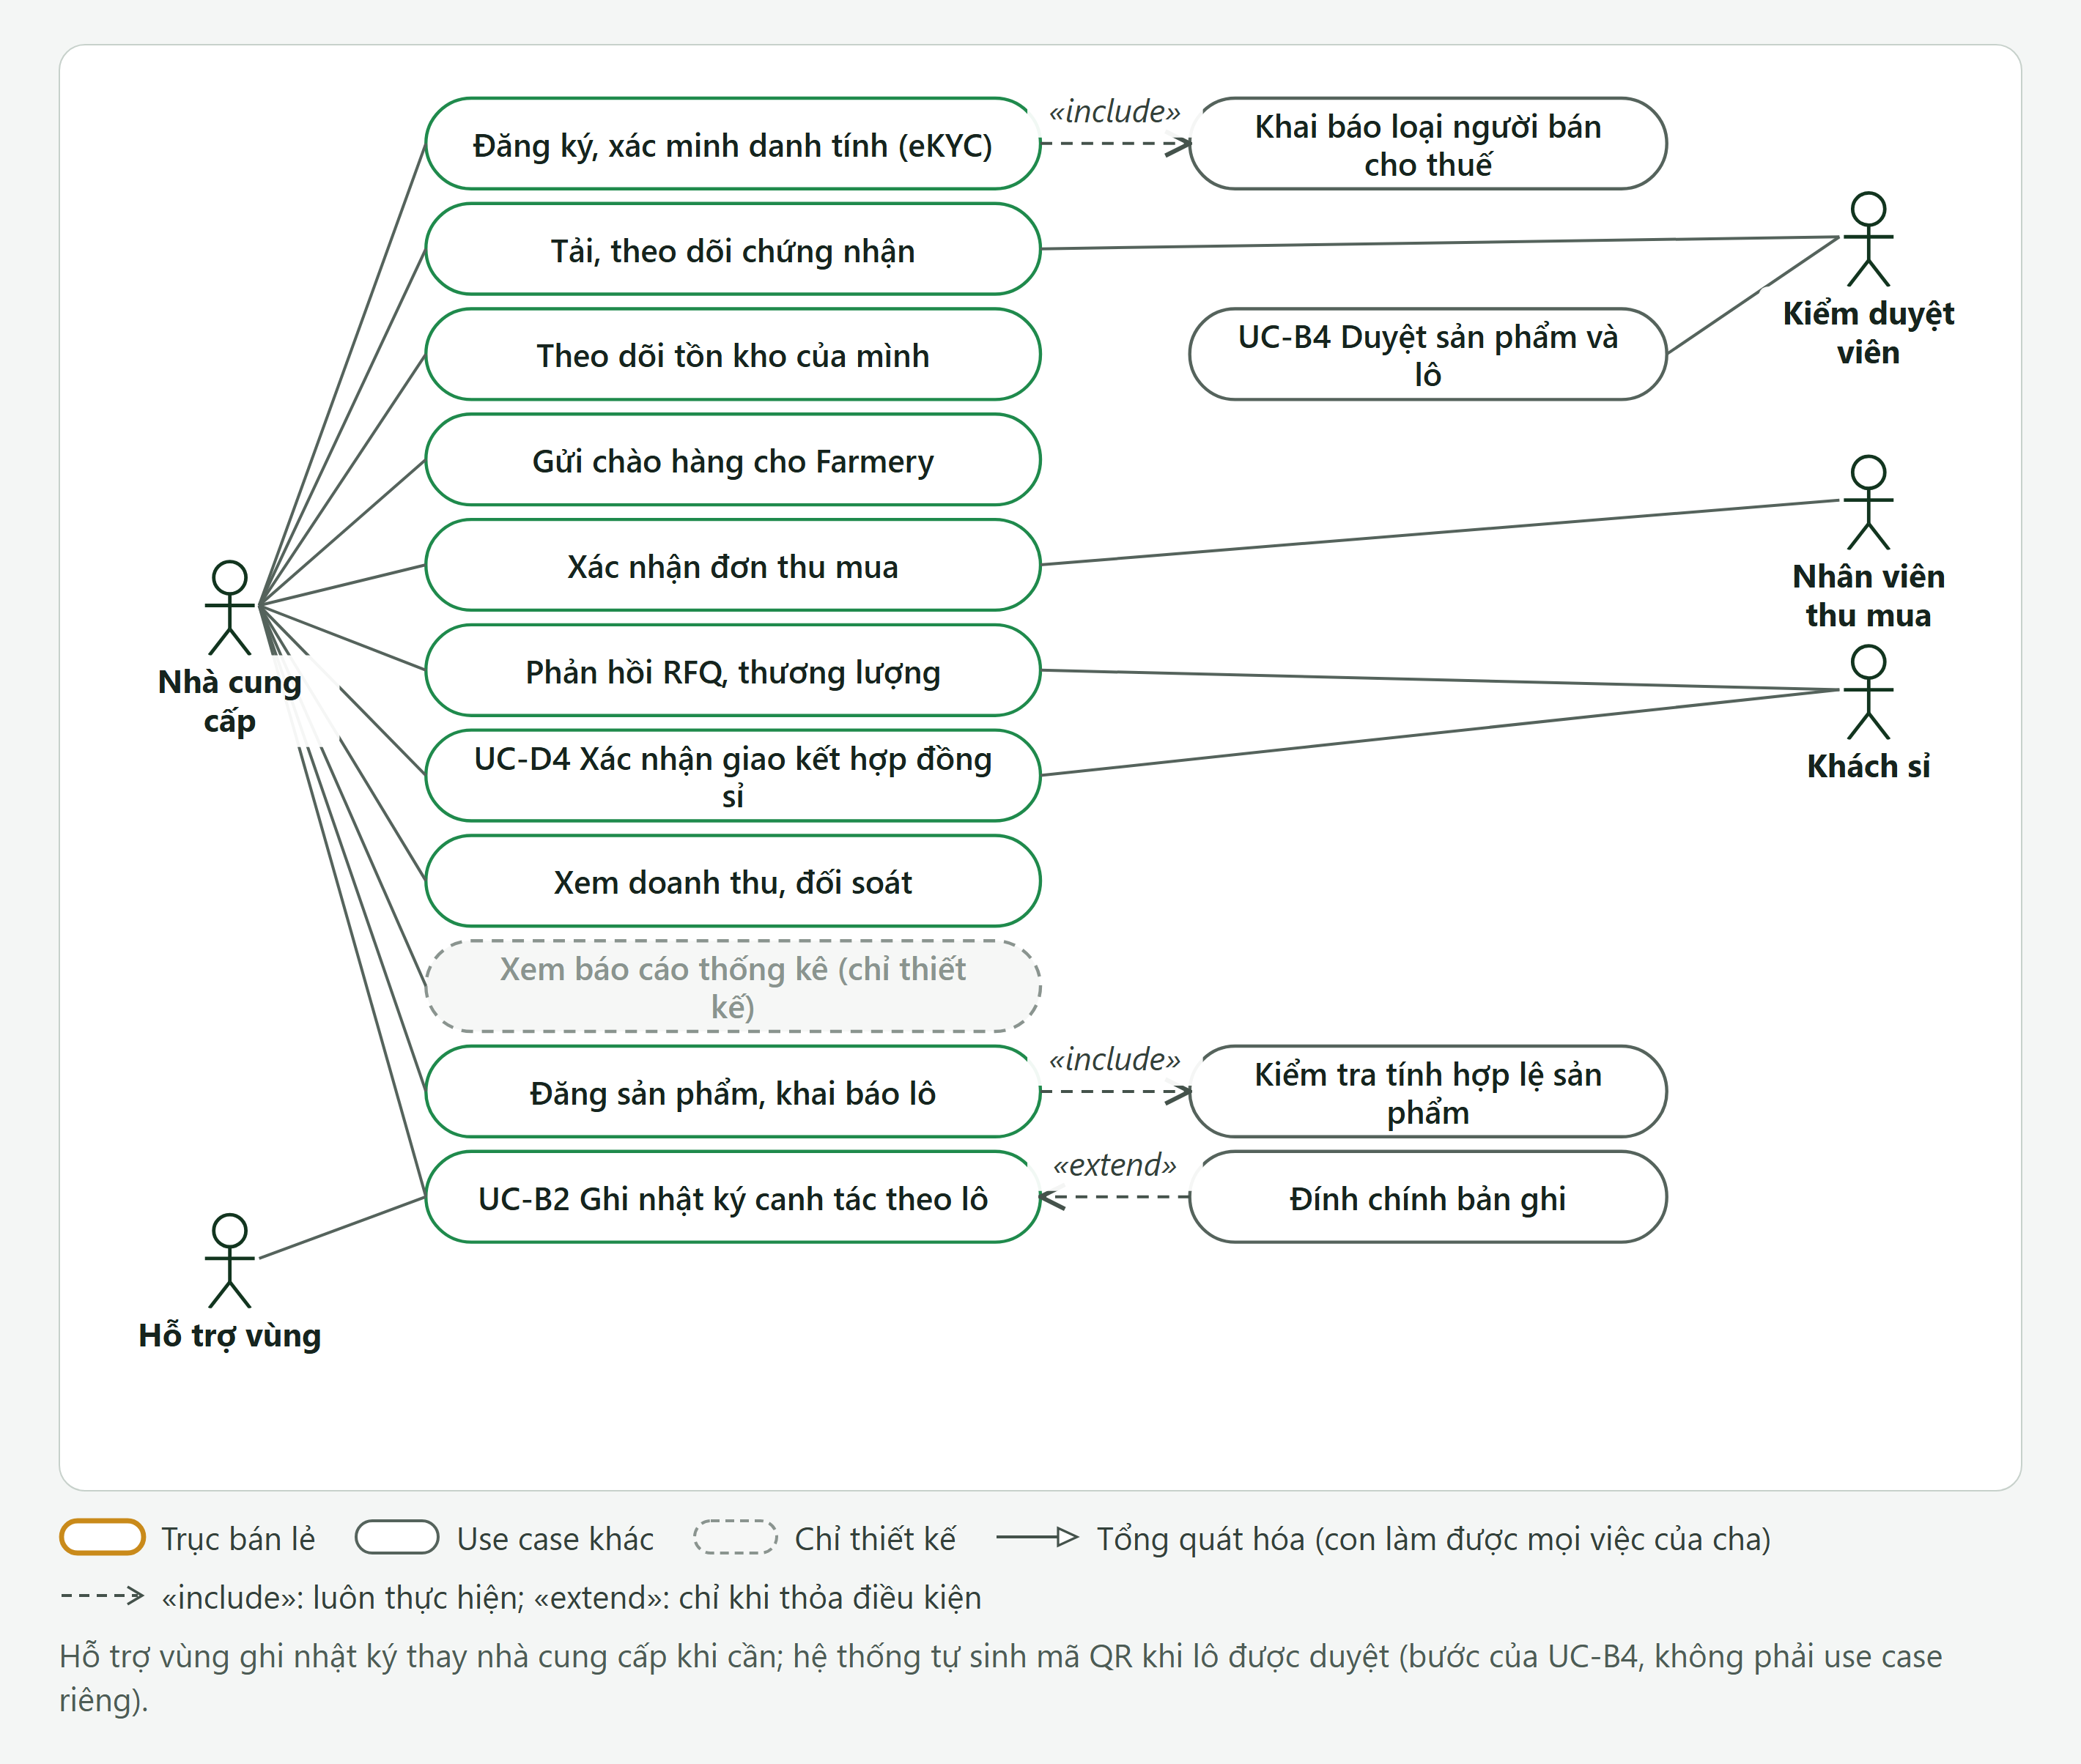
\includegraphics{image/comparison/usecase-nha-ban.png}
\end{adjustbox}
\caption{Sơ đồ Use Case chi tiết --- tác nhân Nhà cung cấp}
\label{fig:usecase-nhaban}
\end{figure}

\begin{figure}[p]
\centering
\begin{adjustbox}{max totalsize={\textwidth}{\dimexpr\textheight-2.5cm\relax},center}
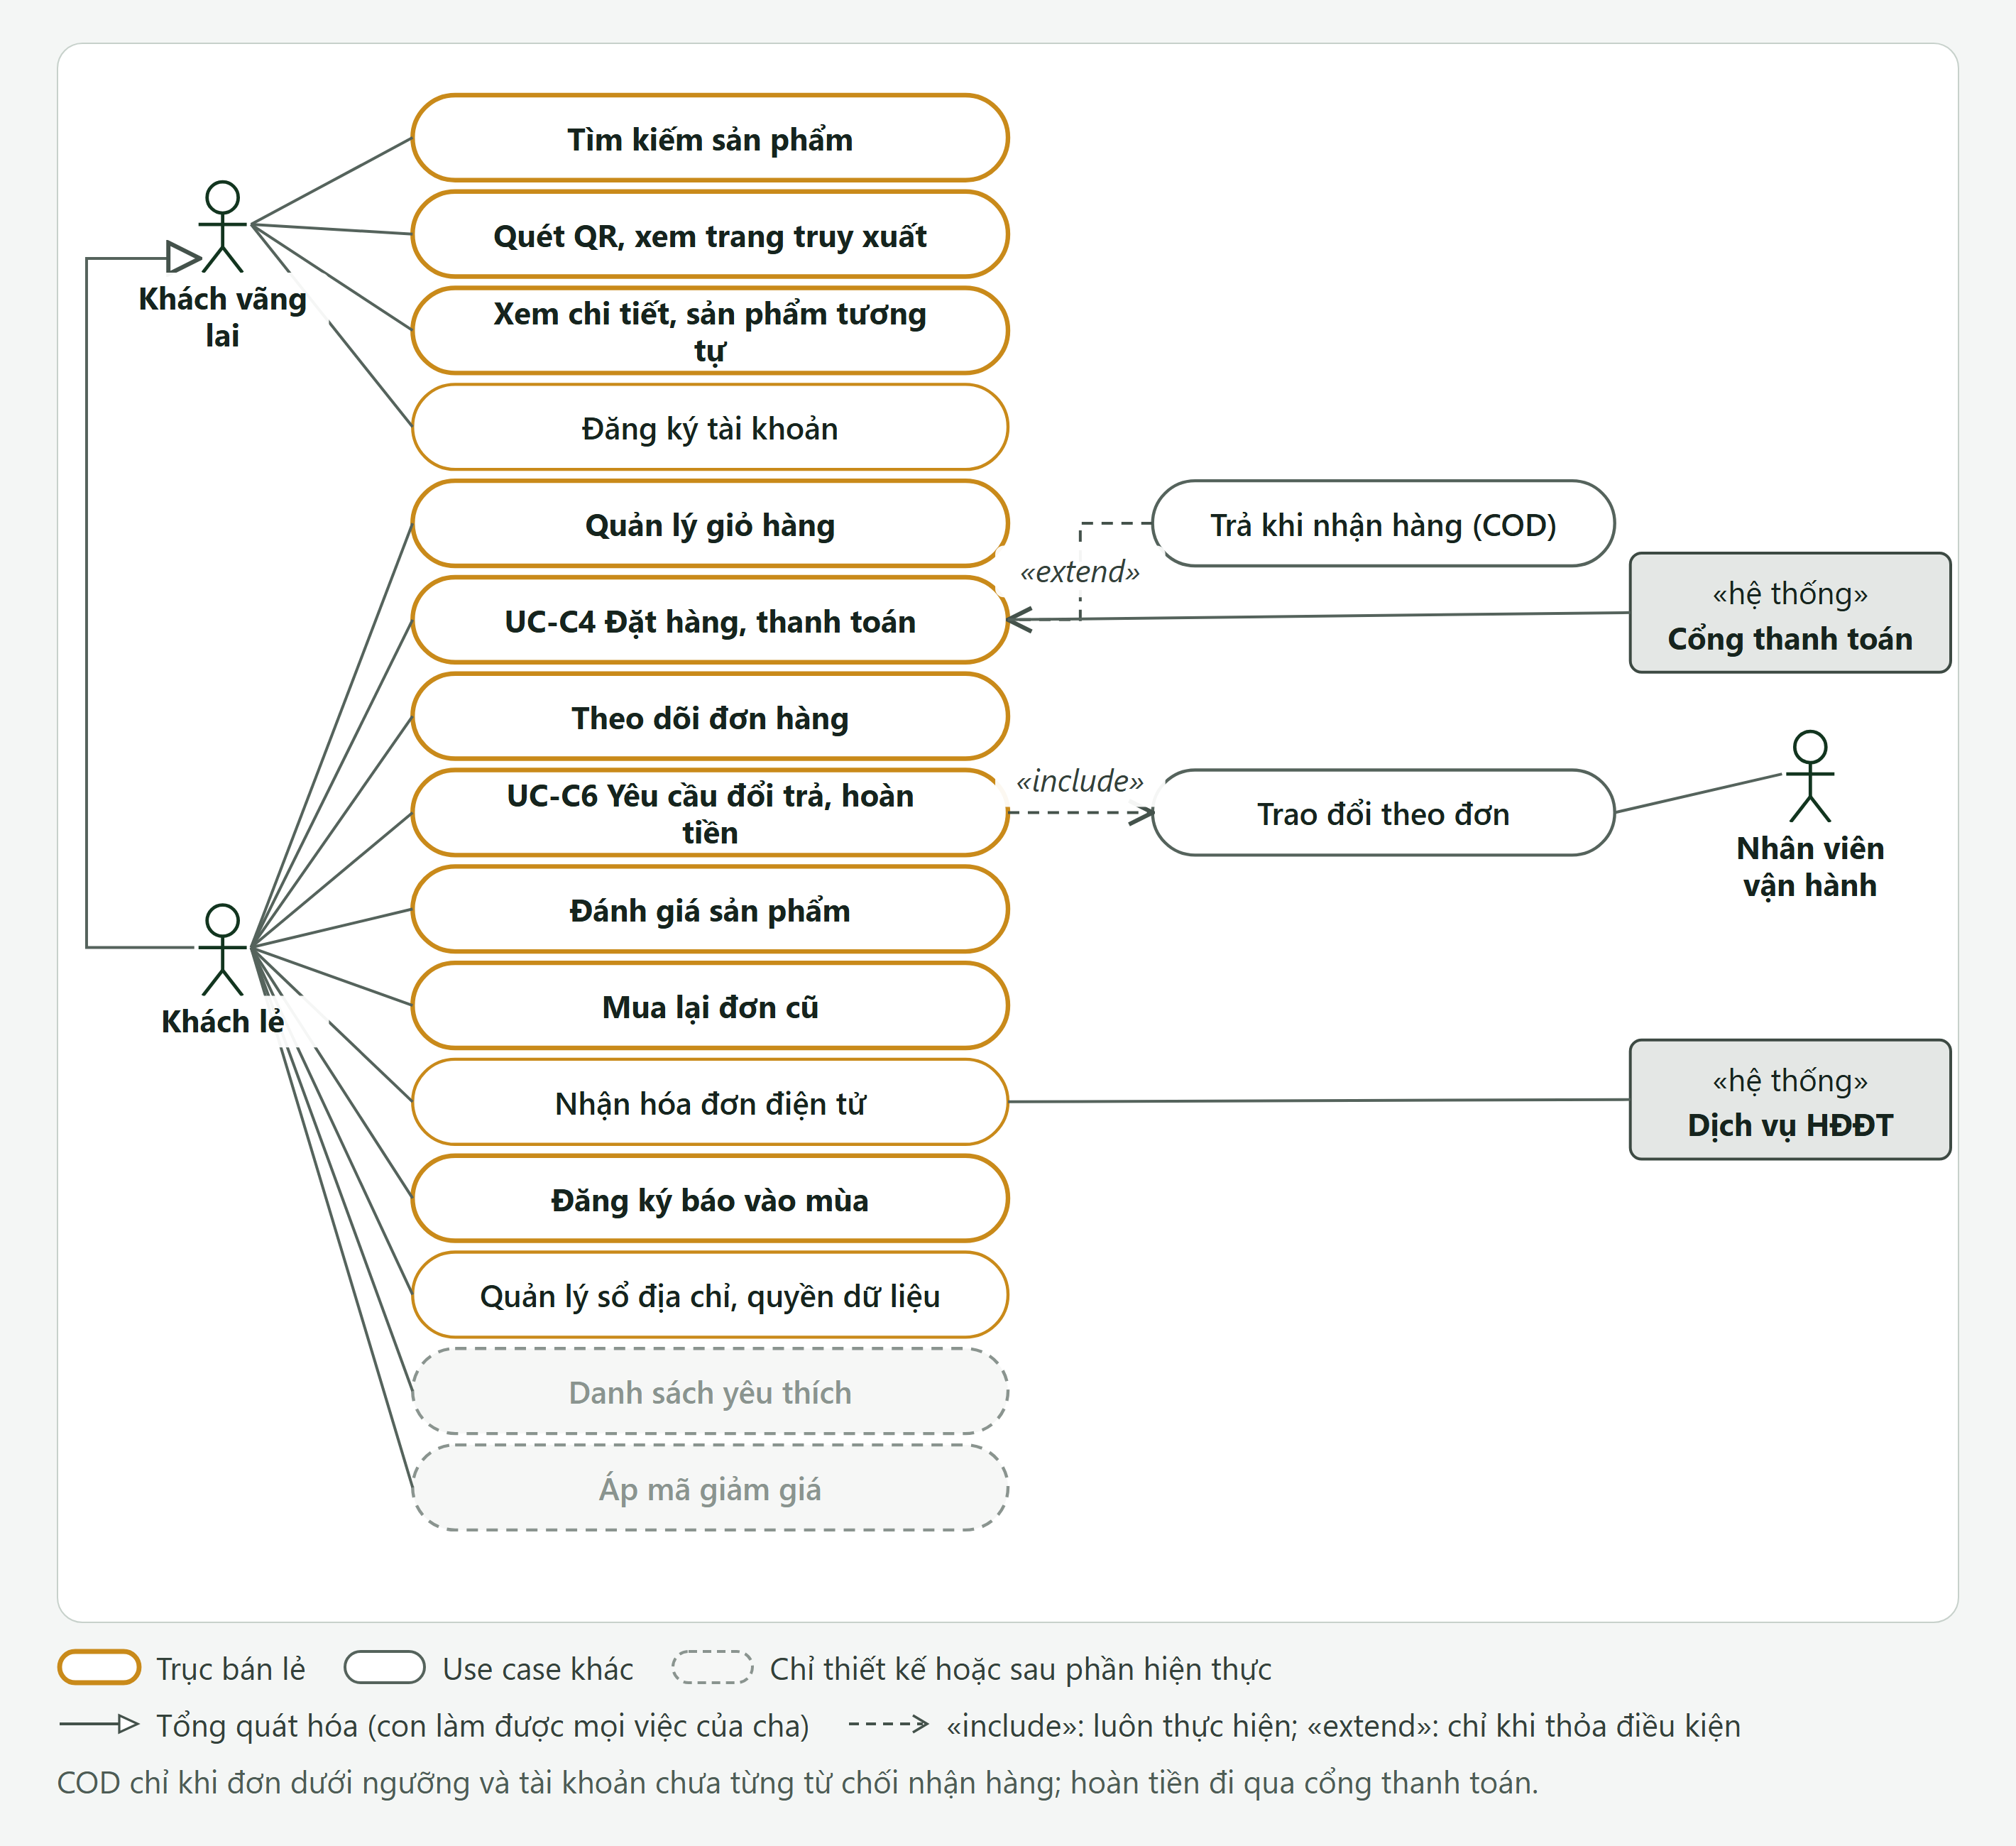
\includegraphics{image/comparison/usecase-nguoi-mua-le.png}
\end{adjustbox}
\caption{Sơ đồ Use Case chi tiết --- tác nhân Khách lẻ}
\label{fig:usecase-khachle}
\end{figure}

\begin{figure}[p]
\centering
\begin{adjustbox}{max totalsize={\textwidth}{\dimexpr\textheight-2.5cm\relax},center}
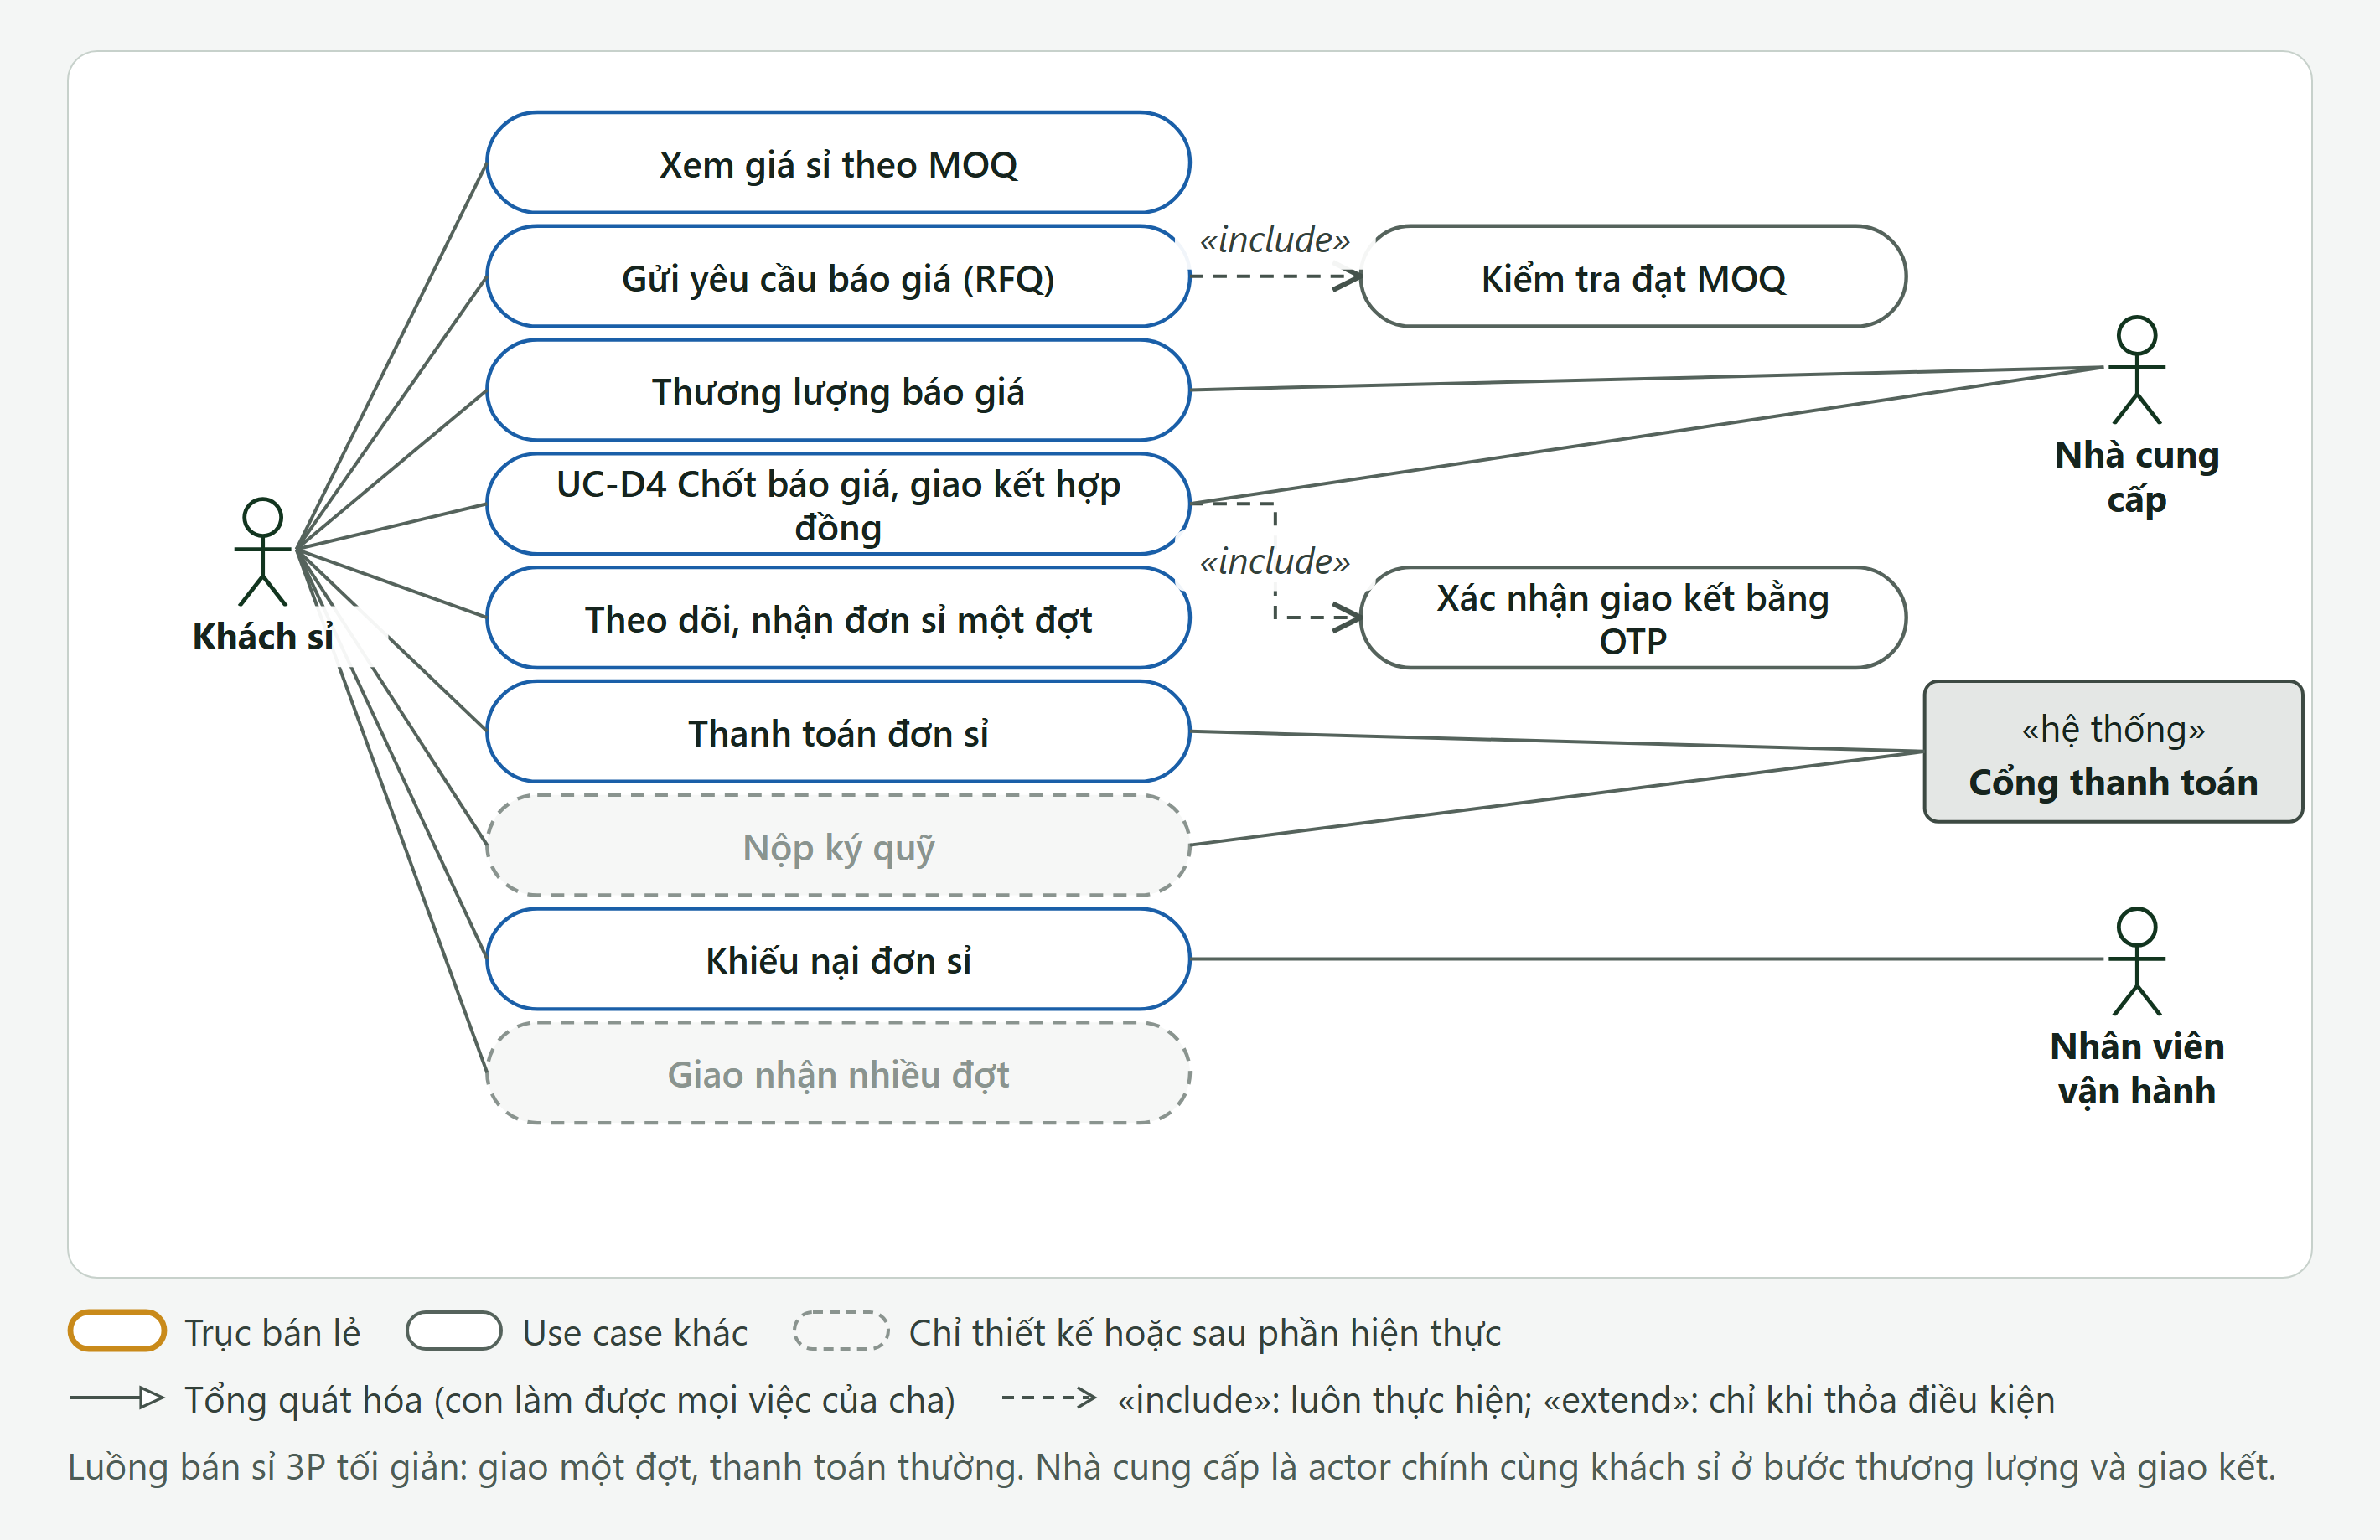
\includegraphics{image/comparison/usecase-nguoi-mua-si.png}
\end{adjustbox}
\caption{Sơ đồ Use Case chi tiết --- tác nhân Khách sỉ}
\label{fig:usecase-khachsi}
\end{figure}

\begin{figure}[p]
\centering
\begin{adjustbox}{max totalsize={\textwidth}{\dimexpr\textheight-2.5cm\relax},center}
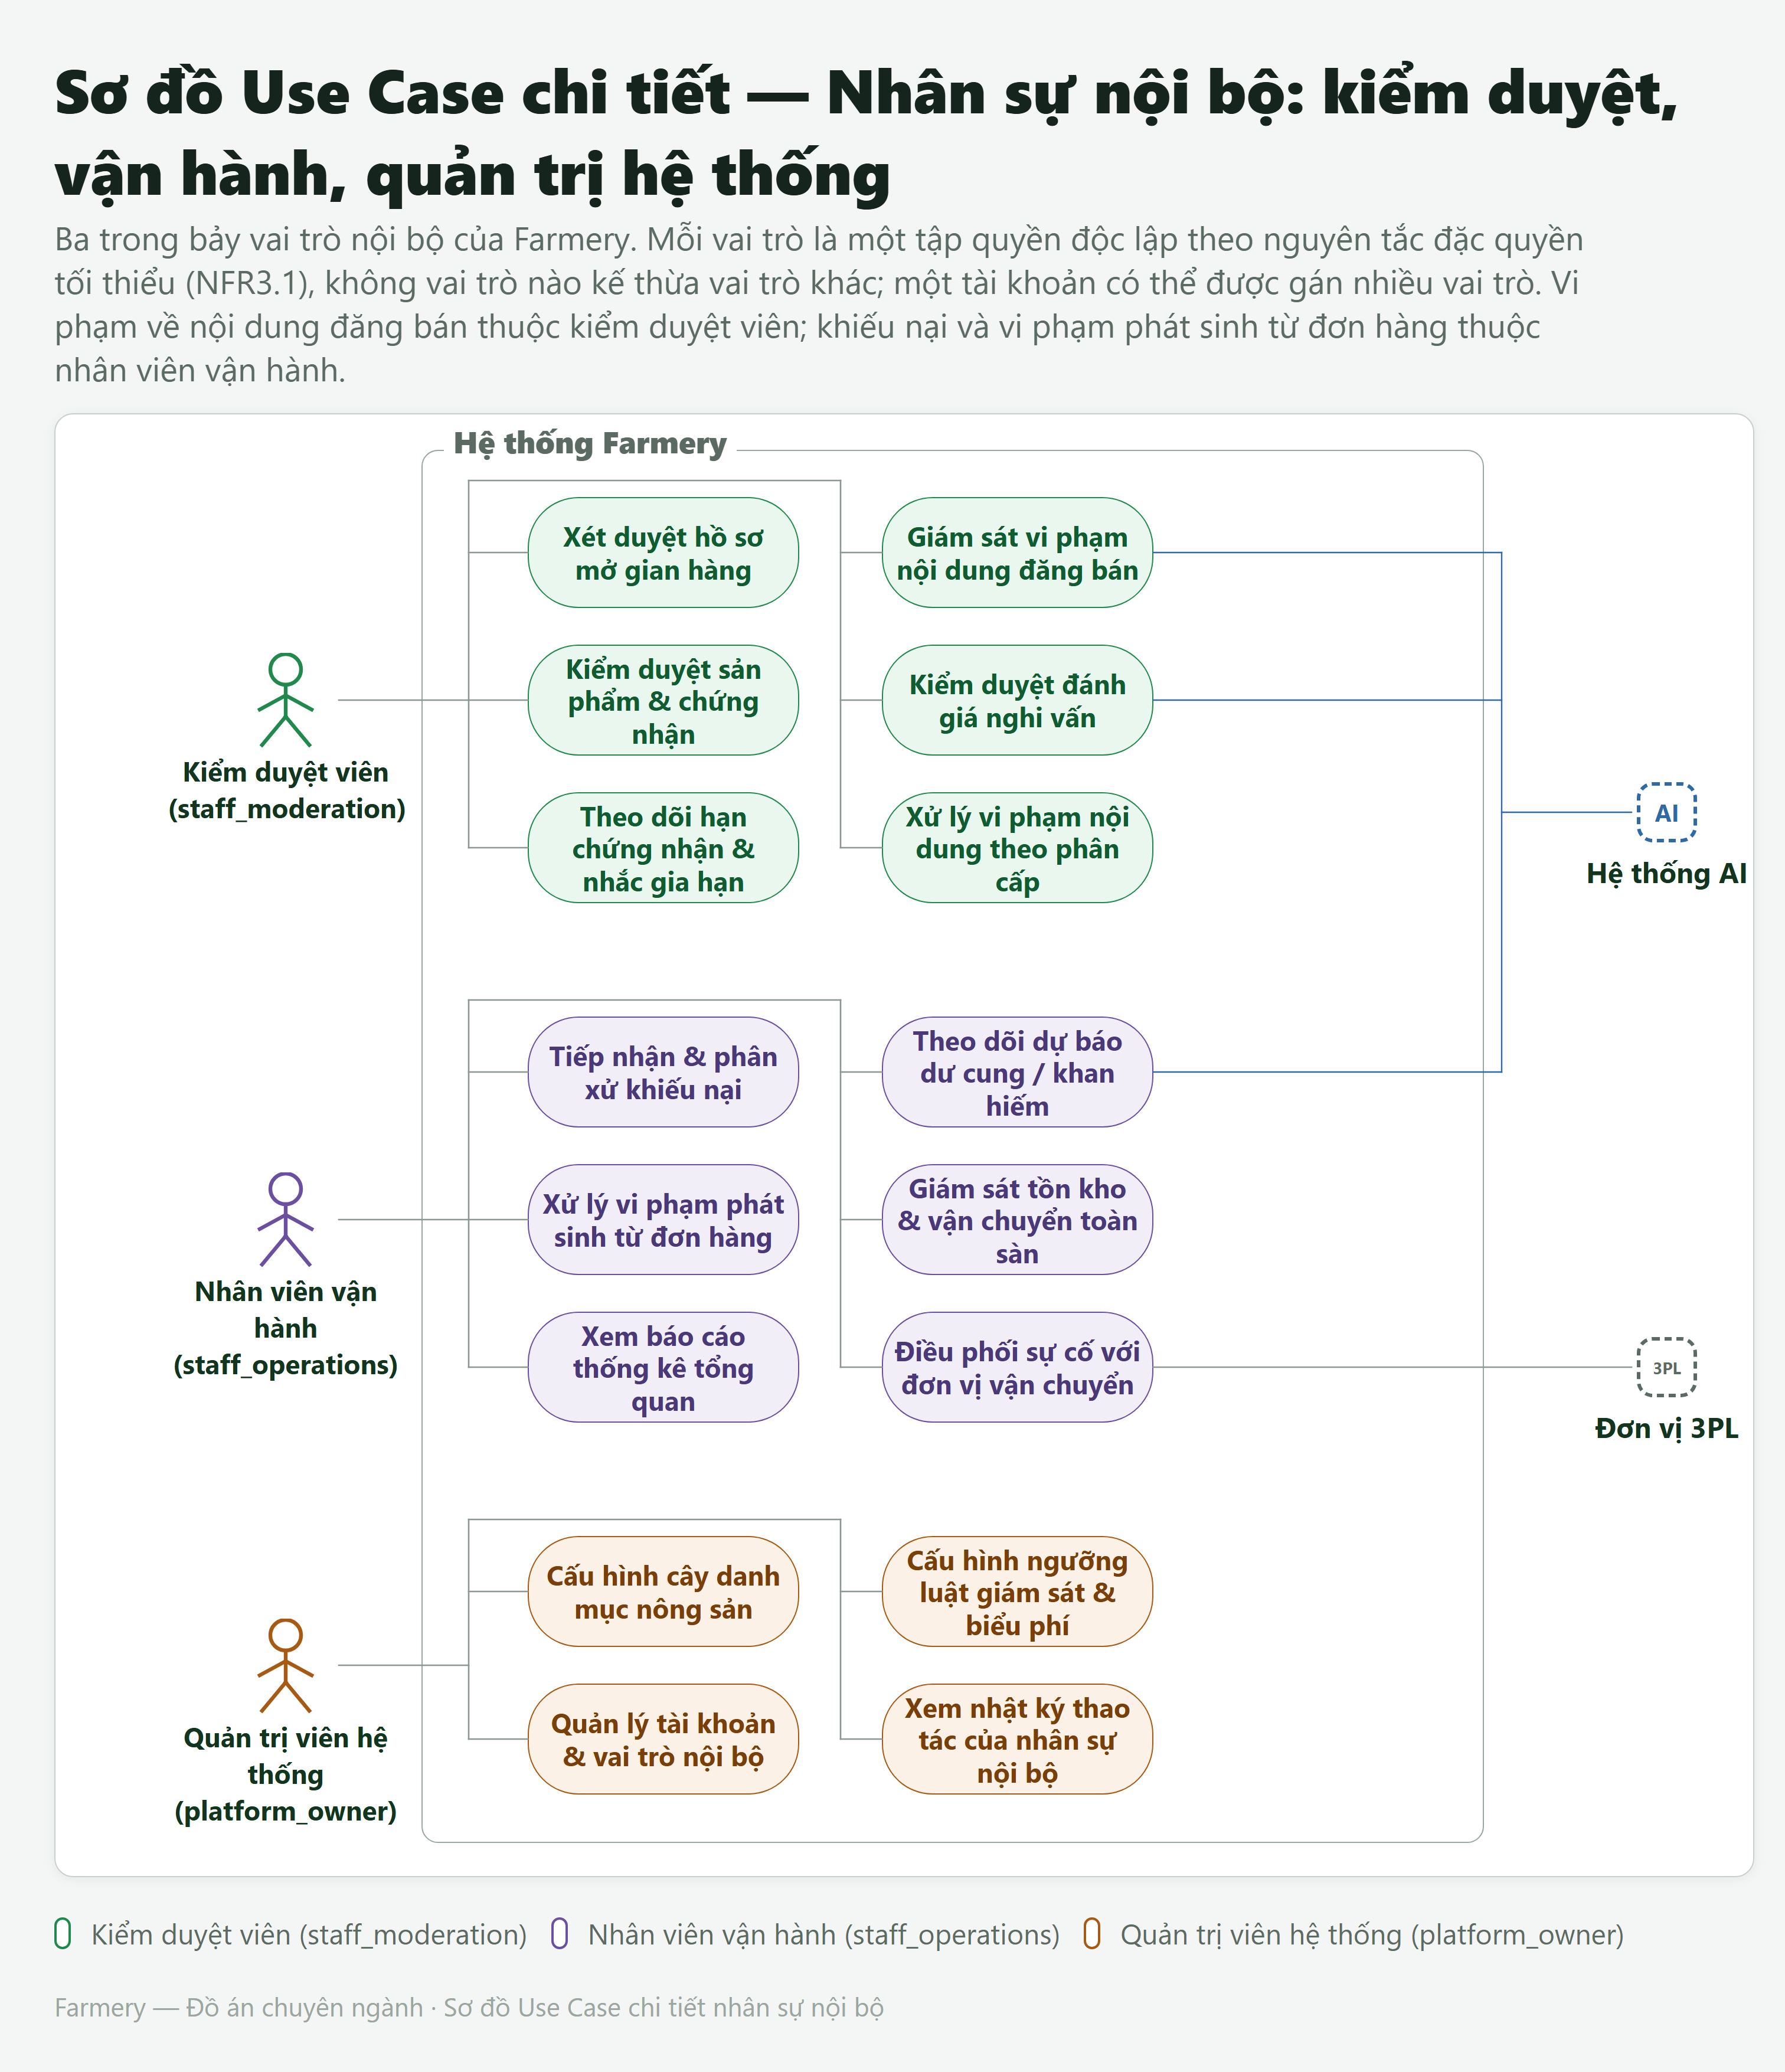
\includegraphics{image/comparison/usecase-quan-tri-vien.png}
\end{adjustbox}
\caption{Sơ đồ Use Case chi tiết --- nhân sự nội bộ (kiểm duyệt viên, nhân viên vận hành, quản trị viên hệ thống)}
\label{fig:usecase-quantri}
\end{figure}

\begingroup
\tblsetup
\begin{longtable}{L{3.00cm} L{12.25cm}}
\caption{Đặc tả use case UC-B2 --- Ghi nhật ký canh tác theo lô}
\label{tab:uc-b2} \\
\toprule
\rowcolor{tblheadbg}
\multicolumn{2}{l}{\textbf{UC-B2: Ghi nhật ký canh tác theo lô}} \\
\midrule
\endfirsthead
\bottomrule
\endfoot
\textbf{Actor chính} & Nhà cung cấp (\texttt{seller}) \\
\textbf{Tiền điều kiện} & Nhà cung cấp đã xác thực (trạng thái ``Đã xác thực''); đã tạo sản phẩm/lô hàng tương ứng (UC-B1) \\
\textbf{Luồng chính} &
1. Nhà cung cấp chọn lô hàng cần ghi nhật ký.\newline
2. Nhập giai đoạn canh tác (gieo trồng/chăm sóc/thu hoạch), ngày tháng, mô tả hoạt động.\newline
3. Tải ảnh minh chứng (nếu có).\newline
4. Hệ thống lưu bản ghi, gắn với lô tương ứng, đánh dấu thời điểm tạo (bất biến, không cho sửa trực tiếp --- NFR9.1).\newline
5. Nếu đủ điều kiện tối thiểu ($\geq$1 bản ghi + ảnh sản phẩm thật), chuyển sản phẩm sang trạng thái đủ điều kiện xét duyệt công khai (UC-B4). \\
\textbf{Luồng thay thế/ngoại lệ} &
4a. Cần đính chính bản ghi cũ: hệ thống không cho sửa trực tiếp, chỉ tạo bản ghi mới kèm ghi chú đính chính (NFR9.1). \\
\textbf{Hậu điều kiện} & Bản ghi được lưu vĩnh viễn (append-only), sẵn sàng hiển thị trên trang truy xuất công khai sau khi sản phẩm được duyệt. \\
\end{longtable}
\endgroup

\begingroup
\tblsetup
\begin{longtable}{L{3.00cm} L{12.25cm}}
\caption{Đặc tả use case UC-D7 --- Xác nhận nhận hàng và thanh toán theo đợt}
\label{tab:uc-d7} \\
\toprule
\rowcolor{tblheadbg}
\multicolumn{2}{l}{\textbf{UC-D7: Xác nhận nhận hàng và thanh toán theo đợt}} \\
\midrule
\endfirsthead
\bottomrule
\endfoot
\textbf{Actor chính} & Khách sỉ (\texttt{buyer\_wholesale}) \\
\textbf{Actor phụ} & Cổng thanh toán trung gian \\
\textbf{Tiền điều kiện} & Nhà cung cấp đã giao hàng đợt tương ứng theo hợp đồng đã ký; hệ thống đã sinh hóa đơn cho đợt giao đó \\
\textbf{Luồng chính} &
1. Kiểm tra và xác nhận đã nhận đủ hàng đúng cam kết của đợt giao.\newline
2. Thanh toán theo kỳ hạn công nợ đã thỏa thuận.\newline
3. Nếu hợp đồng có ký quỹ: hệ thống ra lệnh cho cổng thanh toán giải ngân cho nhà cung cấp ngay tại bước xác nhận này.\newline
4. Nhà cung cấp theo dõi doanh thu/lịch sử bán sỉ cập nhật. \\
\textbf{Luồng thay thế/ngoại lệ} &
1a. Không giao đủ số lượng/đúng lịch: áp dụng điều khoản phạt, ghi vào lịch sử uy tín.\newline
2a. Chậm thanh toán quá hạn: nhắc tự động, có thể tạm khóa quyền đặt RFQ mới.\newline
3a. Phát sinh tranh chấp về đợt giao đã ký quỹ: khoản ký quỹ giữ nguyên tại cổng thanh toán cho đến khi khiếu nại xử lý xong. \\
\textbf{Hậu điều kiện} & Đợt giao chuyển trạng thái hoàn tất, công nợ cập nhật, tiền giải ngân cho nhà cung cấp (nếu có ký quỹ). \\
\end{longtable}
\endgroup

\begingroup
\tblsetup
\begin{longtable}{L{3.00cm} L{12.25cm}}
\caption{Đặc tả use case UC-C7 --- Kiểm duyệt đánh giá nghi vấn}
\label{tab:uc-c7} \\
\toprule
\rowcolor{tblheadbg}
\multicolumn{2}{l}{\textbf{UC-C7: Kiểm duyệt đánh giá nghi vấn}} \\
\midrule
\endfirsthead
\bottomrule
\endfoot
\textbf{Actor chính} & Kiểm duyệt viên (\texttt{staff\_moderation}) \\
\textbf{Actor phụ} & Hệ thống (luật ngưỡng giám sát bất thường, Chương~\ref{chap:coso}) \\
\textbf{Tiền điều kiện} & Người mua đã gửi đánh giá sau khi xác nhận nhận hàng \\
\textbf{Luồng chính} &
1. Kiểm duyệt tự động sơ bộ (từ khóa cấm, liên kết đáng ngờ).\newline
2. Áp dụng luật ngưỡng để tìm dấu hiệu giả mạo/spam/thao túng uy tín.\newline
3. Không nghi ngờ: công khai ngay.\newline
4. Bị nghi ngờ: chuyển kiểm duyệt viên xem xét thủ công.\newline
5. Quyết định công khai hoặc ẩn.\newline
6. Cập nhật điểm uy tín tổng hợp (không tính đánh giá bị ẩn). \\
\textbf{Luồng thay thế/ngoại lệ} &
5a. Xác nhận đánh giá giả/vi phạm: ẩn, thông báo lý do, không tính điểm uy tín.\newline
5b. Phát hiện nhà cung cấp thao túng đánh giá: chuyển quy trình xử lý vi phạm (mục~\ref{sec:quytrinhnghiepvu}, Quản trị hệ thống). \\
\textbf{Hậu điều kiện} & Đánh giá ở trạng thái công khai hoặc ẩn dứt điểm; điểm uy tín cập nhật chính xác. \\
\end{longtable}
\endgroup
